\subsection{Motivating Example: AES encryption algorithm.}

\stefan{I think this example can be trimmed quite a bit. Do you want me to give it a try?}

% We consider a table-based AES encryption algorithm as an example.
%
Advanced Encryption Standard (AES) is one of the most popular encryption algorithms.
%
Given a cipher key, the AES algorithm applies iterative rounds of transformations  to encrypt a confidential input (plaintext) such as passwords and private messages into the ciphertext.
%
The iterative transformations are done sequentially, with the same set of commands, except the last round, which is slightly different. 
%
Each round also transforms the cipher key based on a key schedule; we use the term {\em round key} to refer to the key for each round.
%
AES is a symmetric-key algorithm, meaning that the same key used in the decryption, i.e., anyone who knows the cipher key can deduce the confidential plaintext from the cipher text. 
%
The same key is used to decrypt the ciphertext back to the original plaintext.

AES is a block cipher algorithm that works on fixed-sized blocks of 128 bits.
%
This means that the transformations apply on fixed-sized blocks of 128 bits.
%
Each block of the plaintext is encrypted separately.
%
The block is a 4 x 4 two-dimentional array which we call the input state and is transformed into another 4 x 4 array  which we call the round output state.
%
The output state of one round will be the input state of the next round.
%

\farzaneh{put the transoformation for one round.}

Since the transformations are the same in all blocks, they can be summarized in T-look up tables.
%
For each round, it reads each byte of the input state and use it as the index to the look up key to get T(x), then it uses * to calculate the output state. 
%
All rounds use the same T-look up table, except the final round which is slightly different.
%
y. To speedup the process,
pre-computed tables are used and each round can be implemented with a sequence of table lookups and bit-wise XOR
operations with the round keys, which are expanded from
the 128-bit key
The output of one round is used as indices of the table lookups in the next round, except for the
fnal round, whose output is the ciphertext.
Each AES round can be implemented using four lookup
tables and XORs only, avoiding the expensive polynomial multiplications under.
his approach significantly accelerated
the computation, at the cost of larger memory space required: it
requires four lookup tables each using 256 x 4 bytes

The fundamental reason is that the correlation between the degrees of memory un-coalescing/bank
conficts and the execution time leaks the table index information through the timing channel.
%
n, it is also known that
the table-based AES leaves key-dependent footprints in data
caches, thereby becoming vulnerable to prime-and-probe attacks [21], aka access-driven cache attacks [14, 18],
The input state of each round depends on the plain text and the input state of the previous round and the round key.
%
Consider the final round, for example,

Input to round 10:

8fe5e78f0fd14cf77c816b55e8cce57f



so that they can only be accessed by the parties with high enough security clearance.
%
AES encrypts a data block of length 128-bits storing confidential data.
% 
In AES, a key (which can be a word or phrase) is used to encrypt the plain text data to cipher text and the same key is used to decrypt the ciphertext back to the original plaintext.
%
The plain text cannot be read by any other party except those that possess the key.
%
The encryption phase of AES is applied on each data block of 128 bits by running the same set of steps in iterative rounds.
%
\farzaneh{on each byte of the block}
% It applies 10, 12, or 14 rounds in algorithm and the key can be of size 128, 192, or 256 bits depending on the number of rounds.
% AES is an iterated symmetric block cipher, which means that AES works by repeating the same defined steps multiple times.
%
For a plain text of large size, the GPU parallel pardigm can significantly increase the speed of each round of encryption by applying the steps of a round on all blocks of the plaintext simultaneously (the AES encryption algorithm can be easily parallelized).
%
\farzaneh{and all bytes of the same block.}
The algorithm does the exact same thing to each block.


We consider a table-based implementation of the encryption algorithm in which the steps of each round is summarized as a lookup table.
%
The algorithm reads a block from the memory, for each byte of the block, it calculates an index and looks up the look up table for that index, and replace the byte with a bitwise XOR of the value stored in the look up table and the round key.
%
Since T-tables are constant data and shared by all threads, they are an excellent candidate to store in the shared memory. We assume look up tables are stored on shared memory.
%
\farzaneh{each thread can perform the steps of the round for each byte.}

What indices of the T-tables will be accessed depends on the output text from the previous round which in turn (ultimately) depends on the previous round key and the original plain text. 
% 
% Each GPU thread encrypts a 16-byte block independently.
%
% We transform the AES encryption procedure into a single
% GPU kernel, where each GPU thread can process one block
% encryption, independently. 
%
% Each block consists of 16 bytes.
%
The attacker targets the last-round key. \farzaneh{I'm not sure why last-round and not one to the last?}
%
The attacker can observe the number of bank conflicts (different accesses to the look up table), and based on that number can deduce information about the round key.
%
The number of bank conflicts depends on the key and the plain text. 
%
For example, by observing the bank conflicts, the attacker can distinguish the following two round keys/plain text.

% (It also depend on the implementation and layout of data on shared memory.)

\begin{figure}[h]
    \centering
    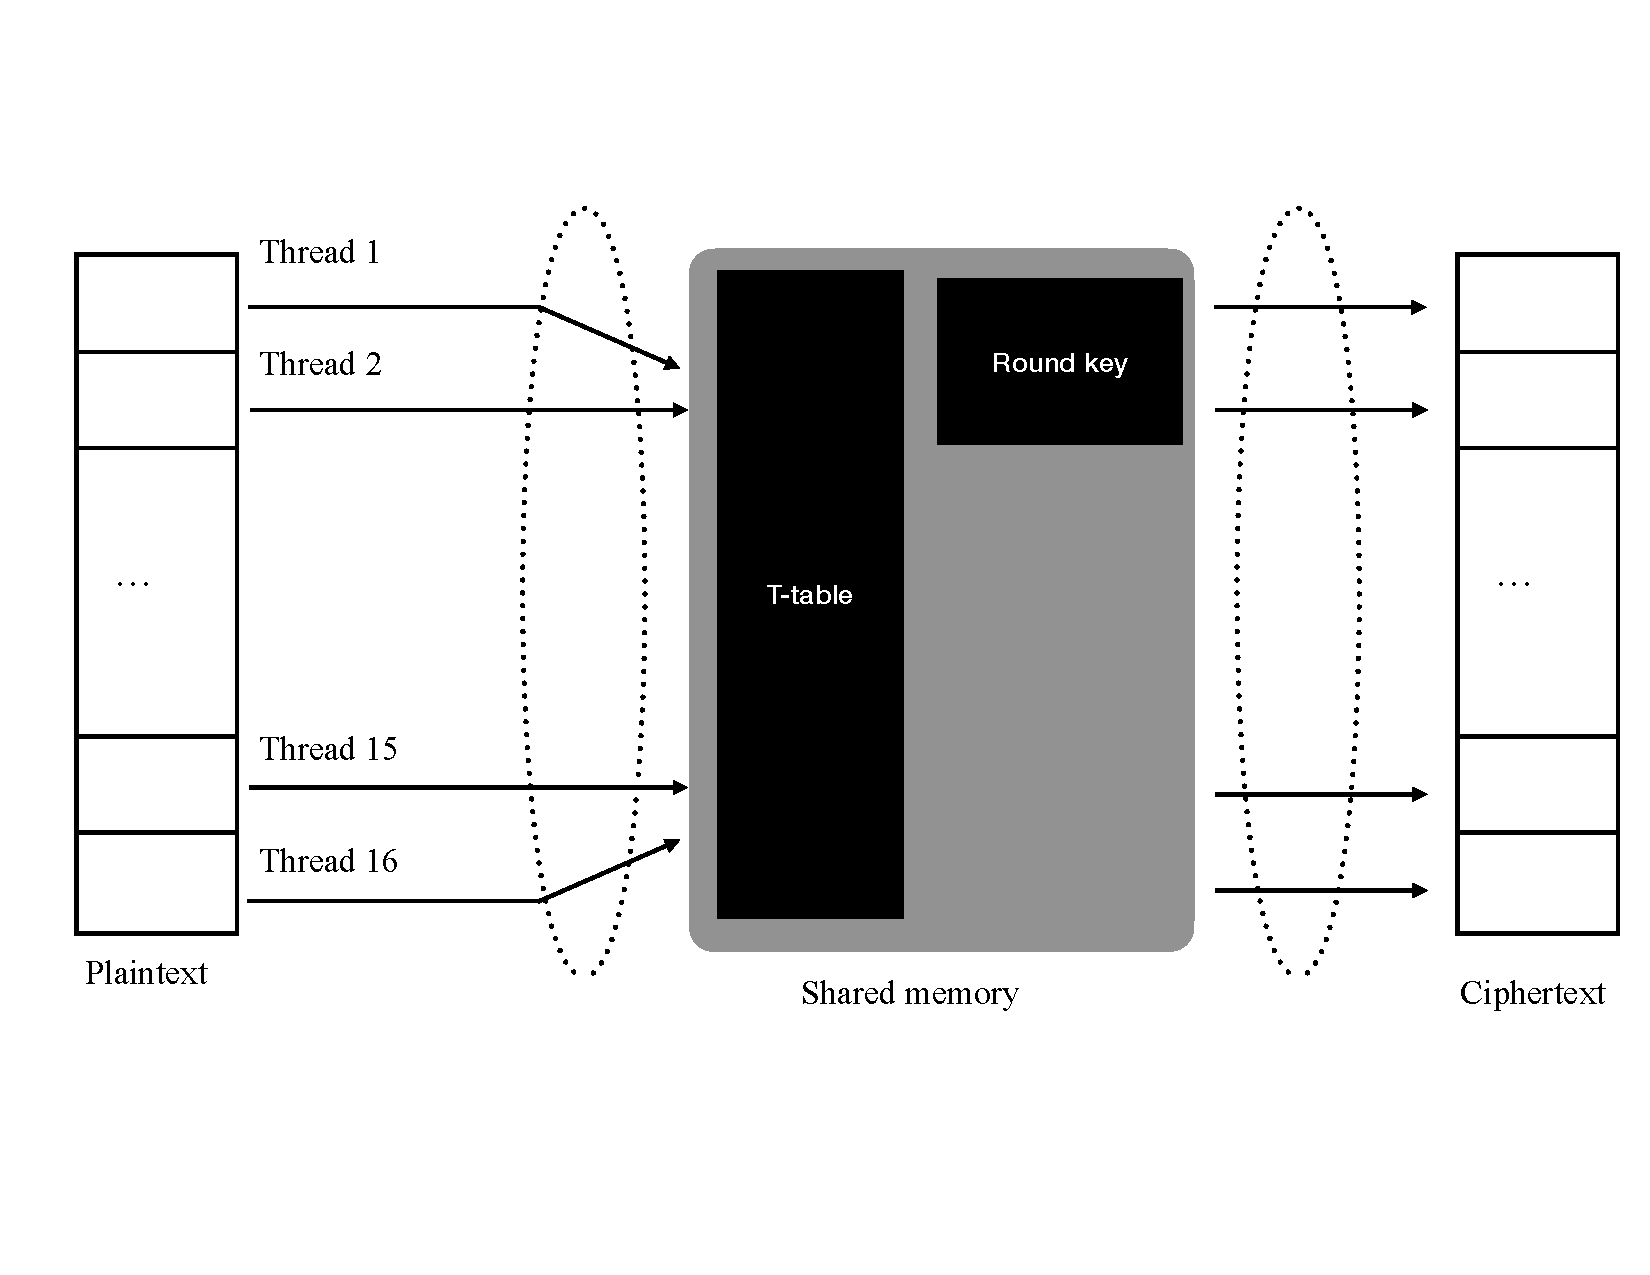
\includegraphics[clip,trim=0 4cm 0 0cm,width=0.7\pdfpagewidth]{figs/AES1.pdf}
    \caption{AES encryption leakage \farzaneh{refine}}
\end{figure}

\farzaneh{Several similar attacks have been described in the literature~\cite{??}.}
\farzaneh{Should we also add coalescing access of Global memory?}
\paragraph{Challenge 1.} The example above is a show-case for the different memory model and parallelism paradigm used in GPU programming. If we naively use the methods developed for CPU parallelism paradigm and its memory model, we cannot capture this new form of side channel attacks.
%
In GPU parallelism paradigm, all threads in one block run the exact same code. 
%
Having different code result in sequentialization of the system which in turn results in different timing behavior. \farzaneh{Maybe the AES example is not the best, because we cannot explain these parts. I'll try to come up with another example.}
%
We need to design a typing system with this memory model and attack model in mind to ensure that we do not leak information.


\farzaneh{move to related work?}This difference has been noticed by several prior work and has been * in attacks. However, the particular solutions that are provided are ad-hoc to each particular exam and are not proved to be correct.
%




\paragraph{Challenge 2.} Avoiding any possible leak is too restrictive and also not realistic. 
%
Small differences in the number of bank conflicts may not even be detectable by the attacker given the undeterministic environment.
%
For example, if the attacker can observe both CPU and GPU runtime (?).
%
Moreover, even if the attacker observes some information it is ok if we leak some sort of information (another reason why LLM is a betetr example).
%
If we be too restrictive and avoid every form of leakage, then we cannot train LLM at all. 
%
What we want however, is to ensure that the information that the attacker observes does not increase its chances a lot for guessing private information enclosed in the training data set.
% The key is fixed. Test it using a given plaintext to find the key.
% Accessing shared memory depends on the key.



%

% AES: shared memory accesses are dependent on the key. 
% %






% As the constant cache stores data
% from constant memory that can be shared by threads
% in a warp, for AES encryption we use this space to store
% round keys.


\subsection{Proposed work}
\subsubsection{Task 1.a. Information Flow Control Type System for GPU Timing Attacks}

Our goal in this task is to statically ensure information security of GPU kernels, and in particular their invulnerability to timing attacks.
%
Our security condition in this task will be {\em cost-sensitive noninterference} \stefan{Is there an existing term for this?} for individual GPU kernels.
%
We define this condition as follows: assign a {\em security level} to every local variable and array in a kernel indicating the secrecy of its contents---for example purposes, we will consider security levels High (high secrecy) and $\bot$ or Low (not secret), but the techniques apply to general lattices of security levels.
%
Consider two executions of a program, starting with memories that agree on variables of security level less than~$\seclevel$ but may differ on higher-security variables.
%
We call such starting points {\em low-equivalent} states.
%
Cost-sensitive noninterference at a security level~$\seclevel$ requires that two executions of a program, starting with low-equivalent states, are indistinguishable in their input-output behavior, effect on low-security memory locations, and observable cost behavior.
%
For most of the examples in this proposal, ``observable cost behavior'' means number of bank conflicts, but in our proposed work, we plan for this to also include number of memory transactions and other performance characteristics closely tied to program data.

In this task, we ensure cost-sensitive noninterference through two main mechanisms.
%
First, we develop a resource-aware Relational Hoare Logic for quantitatively bounding the difference in execution cost between two evaluation of a statement or expression (e.g., that differ only on high-security memory locatins).
%
This logic is sufficient to ensure noninterference and is quite powerful in specifying fine-grained policies.
%
However, it suffers from the same drawbacks as program logics in general: they are often not decidable and require significant human interaction and/or advanced heuristics to prove complex properties such as noninterference.
%
To complement these drawbacks, we will develop an information flow control (IFC) type system that tracks security levels of expressions and statements throughout the program and disallows operations that might violate cost-sensitive noninterference.
%
At key points, for example at a conditional where the condition depends on high-security information, the type system must ensure that the execution costs (e.g., bank conflicts, memory accesses) of the two branches are identical.
%
It does this by ``calling out'' to the Relational Hoare Logic.
%
Uses of the more general logic are therefore localized, reducing the burden on programmers and analysis tools.

We show the soundness of our approach in two steps.
%
First, we show that the Relational Hoare Logic is sound with respect to an operational model of GPU execution.
%
As the model, we plan to use the operational semantics of MiniCUDA~\cite{MullerHo21}, which also track abstract execution cost including bank conflicts and memory accesses.
%
Second, we will show the type system sound with respect to the Relational Hoare Logic, i.e., a well-typed program is related to itself in that any two executions with low-equivalent starting states have the same cost and observable behavior.

\farzaneh{Put more here based on Amal and Jan's RHL.}

A key difficulty in analyzing GPU programs, as opposed to CPU programs, is that each thread maintains a separate copy of local variables.
%
This fact can be used to leak information in non-obvious ways.
%
For example, consider the following program in which~\lstinline{h} is a high-security local variable,~\lstinline{S} is an array stored in shared memory, and~\lstinline{threadIdx} is the integer thread identifier of each thread.

\begin{lstlisting}
if (h) {
  S[2 * threadIdx] = 0;
} else {
  S[2 * threadIdx] = 0;
}
\end{lstlisting}

Naively, it would appear that, although this program conditions on the high-security variable~\lstinline{h}, doing so can't leak information because the code in both branches is identical and the shared memory access uses only low-security indices (\lstinline{threadIdx} is considered low-security).
%
However, the program does indeed leak information.
%
Consider an execution in which threads $0--15$ take the ``then'' branch and threads $16--31$ take the ``else'' branch.
%
In this case, neither branch has a bank conflict, and nor does the program as a whole because the two branches are executed in sequence.
%
On the other hand, consider an execution in which even-number threads take the ``then'' branch and odd-number threads take the ``else'' branch.
%
In this case, both branches have a bank conflict.
%
The leak here is due to the fact that {\em which threads are active} during each branch impacts cost behavior, and this in turn is determined by high-secrecy information.
%

Because GPU programs generally have thousands of threads, reasoning about the local state of individual threads quickly becomes intractable.
%
Muller and Hoffmann~\cite{MullerHo21} observe that a useful middle ground is to instead track which variables are {\em uniform} across all threads and reason precisely only about the local state of these variables.
%
From a cost perspective, this is sufficient in many real-world GPU programs because variables, such as loop indices, that impact cost are generally uniform.
%
We hypothesize that this approximation is useful in a security context as well.
%
For example, in determining that the above program has an information leak, it suffices to know {\em whether}~\lstinline{h} is uniform, because the leak stems from the fact that it may be divergent (i.e., not uniform).
\stefan{Move this example to an earlier section?}

\paragraph{Resource aware - Relational Hoare Logic.}
The judgment for our resource-aware Relational Hoare Logic will be of the form 
%
\[\{\Phi; Q; X\} p_1 \sim p_2 \{\Phi'; Q'; X'\}\]
%
where $p_1$ and $p_2$ are programs the we want to relate (they may be the same program, in which case we relate two executions).%
The logical preconditon $\Phi$  describes the relation between the two states before running programs $p_1$ and $p_2$. 
%
The {\em potential function} $Q$ maps program states to rational numbers.
%
Such a function is familiar from the potential or ``physicist's'' method of amortized analysis, where certain operations accrue potential (analogous to potential energy in physics) in the program state that can then be used to amortize the cost of periodic expensive operations.
%
Our Relational Hoare Logic utilizes a non-standard interpretation of the potential function: the potential actually pays for the {\em difference} between the two execution costs.
%
If the two programs evaluate in lockstep, performing identical memory transactions and other observable operations, no cost is accrued.
%
As discussed earlier \stefan{keep track of where}, we only want to reason about the values of variables that are known to be uniform across all threads; this means that only the states of such variables are included in~$Q$.
%
We keep track of these variables using the third component of the precondition, $X$, which is itself a pair $(X_1, X_2)$ of sets of variables.
%
Sets~$X_1$ and~$X_2$ contain the variables known to be uniform before executing~$p_1$ and~$p_2$, respectively.
%
Moving to the postcondition, $\Phi'$ describes the relation between the two states after running programs $p_1$ and $p_2$; $Q'$ is a potential function for the remaining potential after paying for any differences in cost between $p_1$ and $p_2$, and $X'$ contains the sets of uniform variables in the two executions after executing the two statements.

We will need two forms of rules, {\em synchronous} and {\em unscynchronous}.
%
The synchronous rules relate two executions of the same form of statement;
for example, here is the rule that relates two assignments to shared memory. 
\[
\infer[]{ \Phi[e_1/S_1[o_1]][e_2/S_2[o_2]] \Rightarrow \mathtt{diff\_conflicts}(o_1,o_2) \le n\\  \Phi \vdash e_1 \sim e_2 : m}{\{\Phi; Q+n+m; X\} S_1[o_1] \leftarrow e_1 \sim S_2[o_2] \leftarrow e_2 \{\Phi; Q; X\}  }
\]
The premise~$\Phi \Rightarrow \mathtt{diff\_conflicts}(o_1,o_2) \le n$ indicates that, under the logical conditions in~$\Phi$, it is possible to reason that the difference in the number of bank conflicts between the two indices~$o_1$ and~$o_2$ is less than~$n$.
%
For example, if~$\Phi$ guarantees that~$o_1 = o_2$, then we can conclude~$ \mathtt{diff\_conflicts}(o_1,o_2) = 0$.
%
The auxiliary judgment~$\Phi \vdash e_1 \sim e_2 : m$ states that the difference in the number of bank conflicts triggered by~$e_1$ and~$e_2$ is bounded by~$m$.
%
The rules for this judgment mainly relate shared memory accesses in subexpressions of~$e_1$ and~$e_2$ using~$\mathit{diff\_conflicts}$.
%
In the conclusion of the rule, the main change between the pre- and post-conditions is a cost of~$n + m$ to pay for the maximum possible difference in bank conflicts between the two programs.
%
We also include the information about the assignment in~$\Phi$ by substituting the assigned expressions for the target locations in the precondition, as is standard in Hoare Logic.

The asynchronous rules relate two different forms of statements, and are necessary for, e.g., relating the two branches of a conditional to guarantee that the choice of branch can't leak information through timing channels.

We prove soundness of the Relational Hoare Logic by comparing it to the cost-annotated operational model of CUDA execution developed by Muller and Hoffmann~\cite{MullerHo21}.
%
The operational semantics judgment is~$\sigma; p \Downarrow^{\mathcal{T}}_m \sigma'; n$.
%
In this judgment,~$\sigma$ and~$\sigma'$ are {\em states}, i.e., the values of local variables and arrays, before and after execution.
%
We write~$\Phi \vdash (\sigma_1, \sigma_2)$ to mean that a pair of states satisfies a condition~$\Phi$ in that the states and the relation between them satisfy all of the logical conditions specified in~$\Phi$.
%
The program~$p$ executes with the set~$\mathcal{T}$ of active threads (this may be a subset of all threads if warps have diverged).
%
The judgment also indicates the cost~$n$ of execution in units specified by a {\em resource metric}~$m$, which assigns costs to program operations and conditions---in our example, we would use a resource metric that assigns a cost of~$m$ to an~$m$-way bank conflict and a cost of zero to all other operations.
%
The soundness theorem for the logic states that, if we execute~$p_1$ and~$p_2$ starting with states that satisfy~$\Phi$, the difference in potential predicted by the logic overestimates the actual cost difference between the two executions:

\begin{theorem}[Soundness of Relational Hoare Logic]\label{thm:logic-sound}
If~$\Phi \vdash (\sigma_1, \sigma_2)$ and
$\{\Phi, Q, \{\}\} p_1 \sim p_2 \{\Phi', Q', X'\}$
and $\sigma_1; p_1 \Downarrow^{\mathcal{T}}_m \sigma_1'; n_1$
and $\sigma_2; p_2 \Downarrow^{\mathcal{T}}_m \sigma_2'; n_2$
then $|n_1 - n_2| \leq Q(\sigma_1, \sigma_2) - Q'(\sigma'_1, \sigma_2')$.
\end{theorem}


\paragraph{IFC type system.}
The Relational Hoare Logic described above is sufficient to guarantee noninterferece.
%
We can guarantee that a program~$p$ satisfies noninterference by requiring the
provability of the triple
\[\{\Phi; 0; \{\}\} p \sim p \{\Phi'; 0; \{\}\}\]
where~$\Phi$ is a condition that requires only that the two initial states be low-equivalent.
%
The soundness theorem guarantees that if the triple is provable, then the two executions of~$p$ do not differ in their resource usage.
%
However, proving such a triple may be quite cumbersome and there is no guarantee that doing so would be possible without substantial human effort.
%
We therefore develop a more conservative, but simpler and decidable, type system.

Information flow control (IFC) type systems typically extend conventional type systems by tracking the security level of variables in addition to their data types.
%
In doing so, the type system can, for example, restrict assignments that would
cause high-security information to flow to a low-security variable.
%
In CUDA, we need to track not just the security level of variables and
expressions but also
whether or not they are uniform across threads, because conditioning on
non-uniform expressions can cause leaks, as shown in \stefan{Example}.
%
Types in our type system are~$\tau_{\lpair{\seclevel}{\divergence}}$
where~$\tau$ is a standard data type such as $\mathsf{int}$, and
$\seclevel$ is a security level (we will use~$\bot$ for low-security and~$\top$
for high security; in general these can be values from an arbitrary security
lattice).
%
The component~$\divergence$ is either~$\dunif$ meaning ``uniform across
threads'' or~$\ddiv$ meaning ``possibly divergent (non-uniform) across threads.''
%
We can also treat pairs~$\lpair{\seclevel}{\divergence}$ as elements~$P$ of a
single lattice formed by taking the Cartesian product of the security
lattice with $\{\ddiv, \dunif\}$ and extending the join and ordering operators
in the natural way (uniform values may flow to non-uniform variables but not
vice versa).

Our typing judgment for CUDA statements~$s$ is
$\Sigma, \pc \vdash s$,
where~$\Sigma$ is a context providing the types of constants and variables,
and $\pc$ is the security level of the program counter, which makes the type
system flow-sensitive by indicating whether the control flow of the program
has been influenced by high-security information.


As an example, a general rule for assignments to shared memory might be:
\[
\infer[]
{ \Sigma(S) = \mathsf{arr}(\tau)_{\lpair{\seclevel_S}{\divergence_S}}\\
\Sigma, \pc \vdash o : \mathsf{int}_{\lpair{\bot}{\divergence_o}}\\
\Sigma, \pc \vdash e : \tau_{\lpair{\seclevel_e}{\divergence_e}}\\
(\pc \ljoin \seclevel_e) \secle \seclevel_S
}
{
\Sigma, \pc \vdash S[o] \leftarrow e
}
\]
The assignment is permitted as long as 1) the array index~$o$ is public
(since using a secret index could leak information through the number of
bank conflicts)
and 2) the security level of array~$S$ is at least as high as the
join of~$\pc$ and the security level of~$e$.
%
Clearly~$\seclevel_S$ must be higher than~$\seclevel_e$ as we are writing~$e$
into~$S$.
%
Using the level of the program counter prevents so-called {\em indirect flows}
such as this one, which also writes the value of the boolean~$b$ into~$S[0]$:
\begin{lstlisting}[language=C]
if (b) S[0] = 1;
else S[0] = 0;
\end{lstlisting}

Note that writing to shared memory when the program counter is impacted by
secret information is allowed; disallowing this would be safe, but unnecessarily
restrictive.
%
Instead, we prevent indirect leaks through bank conflicts with the rules
for \texttt{if}.

When conditioning on public information, it suffices to check that both
branches are well-typed:
\[
\infer[]
{\Sigma, \pc \vdash e : \mathsf{bool}_{\lpair{\bot}{\divergence_e}}\\
\Sigma, \pc \vdash s_1\\
\Sigma, \pc \vdash s_2
}
{\Sigma, \pc \vdash \mathsf{if}~e~\mathsf{then}~s_1~\mathsf{else}~s_2}
\]
Note that both branches are typed under~$\pc$ because conditioning on
public information does not increase the secrecy level of the program counter.

However, when conditioning on a secret, we need to ensure that no information
can be leaked through differences in the number of bank conflicts between the
two branches {\em or} through differences in the number of bank conflicts in
one branch that might result from differing sets of threads taking that
branch (see \stefan{Example}).
%
The type system lacks the precision to quantify the number of bank conflicts
and so, at this point, it is necessary to use the Quantitative Hoare Logic:
\[
\infer[]
{\Sigma, \pc \vdash e : \mathsf{bool}_{\lpair{\seclevel_e}{\divergence_e}}\\
\Sigma, (\pc \ljoin \seclevel_e) \vdash s_1\\
\Sigma, (\pc \ljoin \seclevel_e) \vdash s_2\\
\{\Phi; 0; \{\}\} s_1 \sim s_1 \{\Phi'; 0; \{\}\}\\
\{\Phi; 0; \{\}\} s_2 \sim s_2 \{\Phi'; 0; \{\}\}\\
\{\Phi; 0; \{\}\} s_1 \sim s_2 \{\Phi'; 0; \{\}\}\\
}
{\Sigma, \pc \vdash \mathsf{if}~e~\mathsf{then}~s_1~\mathsf{else}~s_2}
\]
We require that the number of bank conflicts in both branches is
unaffected by the set of active threads by relating each branch to itself,
and we require that the two branches have the same number of bank conflicts
under any differences in secret information by relating them to each other.

We prove soundness of the IFC type system by showing that well-typed programs
are related to themselves with empty starting potential.
Composing this result with Theorem~\ref{thm:logic-sound} ensures that
two runs
of a well-typed program with low-equivalent starting configurations do not
differ in the number of bank conflicts.

\begin{theorem}[Soundness of Type System]
If~$\Sigma, \bot \vdash p$
and~$\Phi$ is any condition requiring that the two starting configurations
be low-equivalent,
then $\{\Phi, 0, \{\}\} p_1 \sim p_2 \{\Phi', 0, \{\}\}$.
\end{theorem}



% Explain the type system.
% Relational Hoare Logic
% Logical relation

\subsubsection{Task 1.b.}
In Task 1.a. (\farzaneh{add the ref.}) we follow the classical approach of establishing noninterference to enforce security and ensure that no information is leaked to the attacker. This classical approach, however, is not always feasible or realistic. 
%
In a realistic setting, small leaks of information should be tolerated by the system as long as they are limited and do not significantly compromise the secrecy or identity of other parties.
% 
% Sometimes, certain information must be disclosed to a party with lower security clearance, but only in a way that does not significantly compromise the secrecy or identity of other parties. Sometimes, small leaks of information can be tolerated by the system as long as they are limited and do not increase the chance of guessing the secret by far. 
%
% An unreliable environment might induce noise in the observations of the attacker making the attacker unable to distinguish the difference between certain results, as long as the difference is is not ``too much''. 
% %
Even if the attacker observe different number of bank conflicts in two runs of the program, it may not be able to deduce ``too much'' information from it. 
%
% For example, the AES motivating example does not satisfy the noninterference property, since there is a flow of information from the high security information (plaintext) to low security information (cybertext).
% %
% However, this flow is designed in such a way that that 
% For example, because of the noise in the observations of the attacker, it cannot tell the difference between two execution times as long as the difference is ``not too much''. 
% %
% Or even if the attacker can observe the difference, it cannot deduce ``too much information'' from it. 
% %
The precise threshold for “too much'' varies depending on the specifics of the system. 
%
For example, in the motivating AES example, if the encryption key rotatation is set such that after every ten runs a new random key is generated, then leaking one bit of information in every run, cannot leak more than 10 bits of the ciphertext.
%
If we can quantify information leakage, we can compare it with the established threshold to ensure the system does not significantly compromise security.
%
In this task, we plan to maintain a realistic perspective on security by quantifying leaks via the timing side-channel.
\farzaneh{check the example above.}

We illustrate our approach using the example below.
%
The sample code works on a secret $h$ which stores a two bit value.
\begin{lstlisting}
    if (h=00) {
      S[2 * threadIdx] = 0;} 
    else {
      if (h=01) {
        S[threadIdx] = 0;}
      else {
        if (h=10) {
         S[2 * threadIdx] = 0;}
        else {
         S[threadIdx] = 0;}}}
\end{lstlisting}
% in Figure~\ref{fig:qtable}.
Based on the secret $h$, the program sends threads into four branches, in the first and third branches there are no bank conflicts, in the second and fourth branches there will be 16 bank conflicts.
%
The condition of the branch is not divergent, meaning that all threads will execute the same branch, but depending on the value of the secret the branch can be different.
%
We model the value of the secret $h$ as a random variable.
%
For now, let us assume that the probability distribution of the secret is uniform.
%
Meaning that each possible 2-bit secret value $s$ for $h$ has the same probability of $1/4$, i.e., $P(h=s)= 1/4$ for any $s\in S=\{00,01,10,11\}$.
%
The attacker knows this a priori probability, but cannot 
observe the exact secret stored in $h$; it is uncertain about the value of $h$.
%

Min-entropy provides a measure to quantify the amount of  uncertainty of the attacker (\cite{min-entropy}).
%
It is defined as 
$H_\infty(h)=-\log_2\max_s P(h=s)$,
and captures the probability that the attacker correctly guesses the secret in one try.
%
For example, before executing the program, the min-entropy is $H_\infty(h)=-\log_2\max_s P(h=s)= - \log_2 \max_s \{1/4,1/4,1/4,1/4\}= 2$.
%
We can interpret the min-entropy as the probability of the attacker guessing the correct secret is $1/2^{H_\infty(h)}$.
%
When the random variable has the uniform probability, one can rewrite a priori min-entropy as $H_\infty(h)=-\log_2\max_s P(h=s)=-\log_2 |S|$.
%
In this case, we can also interpret it as there are two bits that the attacker needs to know to fully guess the secret.
%

After executing the program, however, the attacker can observe the number of bank conflicts and learn information about the secret based on the number of observed bank conflicts.
%
If the attacker observes zero bank conflicts, then it can immediately rule out the secret having values $01$ and $11$.
%
While, if the attacker observes $16$ bank conflicts, then it can rule out the secret having values $00$ and $11$.
%
In both cases, the attacker can guess the correct secret in one try with $1/2$ chance.
%

Min-entropy can also be used to calculate a posteriori uncertainty of the attacker  (after the observation) using a conditional probability:
$H_\infty(h\mid b)=-\log_2\Sigma_{o\in O} P(b=o) \max_s P(h=s|b=o)$,
where $b$ is a random variable referring to the number of bank conflicts, $o$ is the number of bank conflict observed, and $O$ is the set of possible observations.
%
In our example, we know that the possible set of observations are $O=\{0,16\}$, the probabilities are $P(h=00,o=0)=P(h=01,o=16)=P(h=10,o=0)=P(h=11,o=16)=1$ with the rest of combinations having value $0$.
%
We can calculate the a posteriori entropy as 
\[\begin{array}{ll}
    H_\infty(h\mid b)=&-\log_2\Sigma_{o\in O} P(b=o) \max_s P(h=s|b=o)=\\ &-\log_2 (P(b=0)\max_s P(h=s|b=0) + P(b=16)\max_s P(h=s|b=16))=\\
    &
    -\log_2 (\max_s P(h=s,b=0) + \max_s P(h=s,b=16))=\\
    & 
    -\log_2 (1+1)= 1
\end{array}\]
We can interpret the a posteriori min-entropy as the probability of the attacker guessing the secret correctly after observing the number of bank conflicts is $1/2^{ H_\infty(h\mid b)}= 1/2$

The amount of information leak can be quantified as $\mathsf{leak}= H_\infty(h) - H_\infty(h\mid b)$, which is equal to $2-1=1$ in our example.
%
This means that in the worst case scenario, the run will leak 2 bits of information.


Smith~\cite{smith} showed that in the case where the program is deterministic and the probability of the secret is uniform, the min-entropy can be reduced to $\mathsf{leak}=\log_2 |O|,$ where $O$ is the set of all feasible obsevations. 
%
(for other probability distributions it is $\le \log_2 |O|.$)
%
This shows that the number of observations is key in calculating the min-entropy. 
%
$\{0,3\}$ will leak the same as $\{0,16\}$.

Our proposed noninterference theorem in \ref{task:1a} ensures that no information will be leaked.
%
In other words, if we can prove the noninterference theorem for $s$, aka $\{\Phi;0; \{\}\}s \sim s\{\Phi;0;\{\}\}$, we know that all threads will have the same number of bank conflicts.
%
There is only one feasible observation and thus $\mathsf{leak}\le \log_2 |1|=0.$

% one of the columns is all $1$ and every other column has value $0$.
%
Now let us see what it means if we have $\{\Phi;0; \{\}\}s \sim s\{\Phi;n;\{\}\}$.
%
It states that the differences between the number of bank conflicts in any two runs of the program is capped by $n$.
%
% All columns are the same except $n$ consecuritve columns that can be different.
%
This automatically provides an upper bound $n$ on the number of feasible observations, given that the number of bank conflicts is always a positive natural number. 
%
However, this upper bound in many cases is too generous.
%
For example, for program $s_0$ given above, we have $\{\Phi;0; \{\}\}s_0 \sim s_0\{\Phi;16;\{\}\}$, while we with 0 and 16.
%
We plan to investigate this further by adopting our logic to not only provide an upper-bound but also a set of possible outcomes.
%
The set can (and should for decidability reasons) still be an over-approximation but it can reduce the space further.
%
This will be captured with the diffconflicts premise, instead of measuring the upper bound, it will provide a list of possible differences.
%

After that, we plan to also consider arbitrary distributions other that uniform. 
%
We have to work with the original formula.
%
(no nondeterministic for now).
%
An unreliable environment might induce noise in the observations of the attacker making the attacker unable to distinguish the difference between certain results, as long as the difference is is not ``too much''. 
% Based on the noise of the environment and the abilities of the attacker, we can also say whether two possible observations are distinguishable to the attacker.
% %
% For example $1$ vs $2$ and $2$ vs $3$ is not observable to the attacker.
% %
% But $1$ vs $3$ is.
% \farzaneh{is it a problem that we don't have a transititivity? Add more here.}

% It is defined as as the negative logarithm of the probability of the most likely outcome.

% The guarantees we obtain are upper bounds
% on the amount of information about the input that an adversary can extract by
% observing which memory locations are present in the CPU's cache after execution
% of the program;




% We plan to incorporate quantitative analysis in the RHL, limiting the probability of the leak, e.g., via shared timing attacks, to a set threshold.

% \farzaneh{add a connection to the motivating example:In our motivating example: For each plaintext we get x bits of information about the key.  %
% If we run it multiple times with different plaintext, we can find the key compeltely.   A possible scenario: leaking three bits can be tolerated because after every ten runs a new random key is generated? this is called key rotation.}


  
    % Such theories offer an attractive way to relax the standard noninterference properties, letting us tolerate “small” leaks that are necessary in practice. 
%

% In this task, we plan to maintain a realistic perspective on security by allowing the possibility of leaks as long as they are limited and do not leak too much information. The precise threshold for “too much information” varies depending on the specifics of the system. We define the threshold by incorporating quantitative analysis in the RHL, limiting the probability of the leak, e.g., via shared timing attacks, to a set threshold.


    % In our motivating example: For each plaintext we get x bits of information about the key. 
    % %
    % If we run it multiple times with different plaintext, we can find the key compeltely : Quantitative aspect.
    % %
    % A possible scenario: leaking three bits can be tolerated because after every ten runs a new random key is generated? this is called key rotation.
    % Min entropy.
    % Such theories offer an attractive way to relax the standard noninterference properties, letting us tolerate “small” leaks that are necessary in practice. 


    % A quantitative metric measuring “distinguishability”
    % should account for an optimal guessing strategy employed by the
    % attacker. Such an optimal guessing strategy should guess the most
    % likely victim access pattern by leveraging full knowledge of the
    % obfuscating scheme's probabilistic properties



\subsection{Task 1.c} Implementation of the type system.
Formalizing the proofs.
